\documentclass[ProductRequirements.tex]{subfiles}
\begin{document}

\bigskip

\section{\textsc{\Large Overall Description}}
	\subsection{Product Perspective}
	\begin{figure}[H]
		\centering
		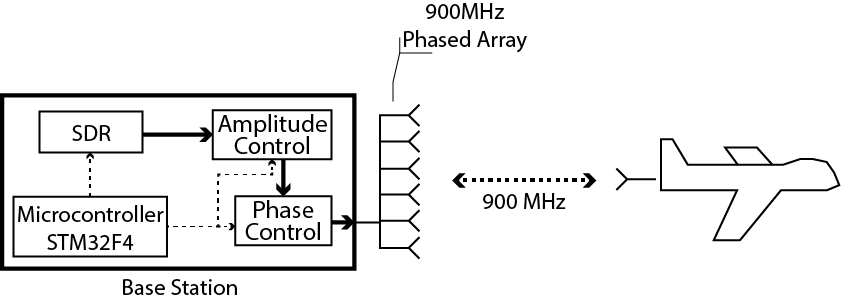
\includegraphics[]{HardwareBlockDiagram.png}
		\caption{Hardware Block Diagram \label{fig:HardwareBlockDiagram}}
	\end{figure}
	\begin{figure}[H]
		\centering
		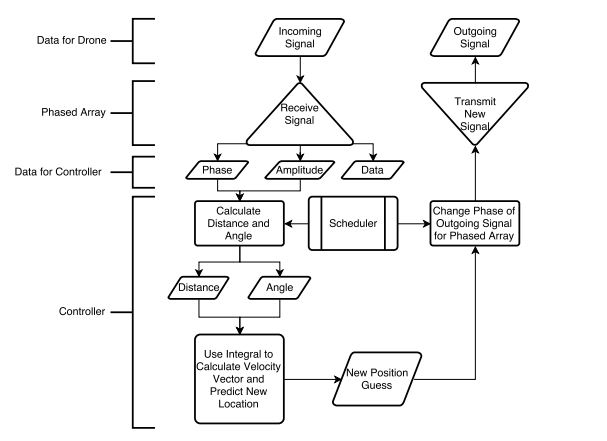
\includegraphics[]{SoftwareBlockDiagram.png}
		\caption{Tracking Block Diagram \label{fig:SoftwareBlockDiagram}}
	\end{figure}
			
		\subsubsection{User Interfaces}
			The system must have an Ethernet port through which the user can establish a connection. The user should be able to modify various settings and send the commands of interest through this port. This port must conform to the following requirements:
			\begin{enumerate}
				\item When a connection is established, the interface must send a list of instructions and changeable parameters over Ethernet.
				\item The interface must be straightforward enough that a technical user can use the instructions to configure the settings within 20 minutes.
				\item There must be clear documentation about each setting describing (1) what it does, (2) why it's valuable, and (3) how to use it.
			\end{enumerate}	
			
		\subsubsection{Hardware Interfaces}
			\begin{enumerate}\itemsep1pt
				\item \textbf{STM32F4} -- The SDR or radio data must be received and piped bidirectionally via the RF chain to the STM32F4 microcontroller via an Ethernet connection.  Additionally, the STM32F4 is responsible for "beam steering," or appropriately setting phase and magnitude to each of the RF elements.  The general purpose input/output pins of the STM32F4 will be used to set the elements. A JTAG header will provide an programming interface to the microcontroller.
				\item \textbf{SDR/Radio} -- The radio is responsible for producing and receiving the modulated signal from the antenna elements.  The radio will communicate with the STM32F4 via an Ethernet connection to ensure a radio agnostic system.  The radio will interface with the elements via a SMA connection.  
				\item \textbf{Phased Array} -- The phased array elements transmit and receive the RF signal from the remote target.  The phased array will interface to the system via the SMA connection to the user's radio of choice.
				\item \textbf{Power Board} -- The power board must supply sufficient power to the entire system.  Power rails will interconnect the boards through high current headers.
			\end{enumerate}
			
		\subsubsection{Software Interfaces}
			\begin{enumerate}\itemsep1pt
				\item \textbf{Tracking Interface} -- A user can interact with, modify, and control the system using an application GUI derived in Python.
				\item \textbf{Packet Structure} -- All data/control must be wrapped into a standardized packet structure for system piping as well as identifying potentially valid connections.
			\end{enumerate}
			
		\subsubsection{Communications Interfaces}
			\begin{enumerate}\itemsep1pt
				\item \textbf{Ethernet} -- Standard Ethernet protocol will be incorporated into the design to allow for radio agnosticism as well as a simple, standardized user interface.
				\item \textbf{ISM Band} -- All radio communications will occupy the 902-928 MHz ISM bands.
			\end{enumerate}
			
		\subsubsection{Memory}
			\begin{enumerate}\itemsep1pt
				\item \textbf{SDRAM} -- External memory will be implemented in the system to allow for data buffering in the case of high volume data transfers.  
			\end{enumerate}
		
		\subsubsection{Operations}
			\begin{enumerate}\itemsep1pt
				\item \textbf{Manual Beam Steering} -- The system should be able to be manually directed by a user.  A user should be able to set the relative or absolute beam direction.  After acquiring the lock the system can be set to automatically track the established target.
				\item \textbf{Automatic Beam Steering} -- The system should be able to automatically acquire drones and establish connections.
			\end{enumerate}
		
	\subsection{Product Functions}
	
		\subsubsection{High Priorities}
			\begin{enumerate}
				\item \textbf{Distance} -- The 900MHz phased array must be able to establish a connection with a drone in motion up to 20 miles away. A connection will be considered valid if we are receiving packets with a valid header.
				\item \textbf{Power} -- The 900MHz phased array must never exceed the FCC maximum power specifications of 4 watts.
				\item \textbf{Command Transmission Rate} -- The 900MHz phased array must be able to transmit telemetry at 10Hz.
				\item \textbf{Cost} -- The product should cost no more than \$10,000 to produce the prototype.
							
			\end{enumerate}
		
		\subsubsection{Medium Priorities}
			\begin{enumerate}
				\item \textbf{Communications} -- The communications should be radio agnostic.
				\item \textbf{Array Refresh Rate} -- The phased array should be able to update all elements at a 100 Hz rate.
			\end{enumerate}
		
		\subsubsection{Low Priorities}
			\begin{enumerate}
				\item \textbf{Multiplexing} -- The phased arrays should be able to simultaneously communicate with up to 4 drones at once while maintaining a lock.
				\item \textbf{Video} -- The system should be able to process and receive high data rates such as a low-latency video feed from the target.
				\item \textbf{Stacked Antennas} -- The 2.4GHz phased array must be able to establish a connection with a drone in motion up to 5 miles away.
			\end{enumerate}
		
	\subsection{User Characteristics}
		We intend to market this product to people who are interested in managing multiple drones at once with lower power at longer distances. Because this is a backend product, the user will be expected to be somewhat familiar with embedded systems. The user should have prior knowledge of SDR and drones. Because the system is radio agnostic, the user will need to supply his own SDR. The user will need to supply data that is compatible with his SDR to our program.\\
		
		The user will not be expected to have familiarity with RF Design, tracking, locking, or our internal headers.
		
	\subsection{Design Constraints}
		\subsubsection{Regulatory Policies}
			\begin{enumerate}
				\item \textbf{Power Limitation} -- The system must conform to the FCC Maximum power specifications
				\item \textbf{Unmanned Aircraft Systems} -- The system must conform to the FAA drone regulations.
			\end{enumerate}
		\subsubsection{Interfaces to Other Applications}
			\begin{enumerate}
				\item The system must be able to interface with all standardized SDRs and radios.  Standardized radios support Ethernet or serial connections.
				
			\end{enumerate}

		
	\subsection{Assumptions and Dependencies}
		\begin{enumerate}
				\item \textbf{FIRST RF} -- We are dependent on FIRST RF for their facilities for design IP and testing.  
				\item \textbf{BlackSwift Technologies} -- We are dependent on BlackSwift Technologies for the use of their drones for the purpose of testing our product.  
				\item \textbf{Xetawave} -- We are dependent on Xetawave for the use and support of their SDR technology for testing our system.
		\end{enumerate}
\end{document}
